
\ifx\penExCode\somethingUndefined

\newcommand\penExCode[2][2.5cm]{%
%\adjustbox{max totalheight=2.5cm,set depth={\dimexpr 2.5cm-\height\relax},
\adjustbox{%left=0.95\textwidth,bgcolor=gray!10!white,
    raise={-\height},set height=0cm,set depth=#1}{%
%		\parbox{\linewidth}{%
%			\hspace{-0.25em}\vrule width \dimexpr 0.95\textwidth+0.25em\relax depth 0px height 5.5px\par
%			\vspace{-\baselineskip}%
%			%
        \adjustbox{
            max totalheight=#1,
        %\adjustbox{max totalheight=2.5cm,min totalheight=2.5cm,raise={\depth},
            %bgcolor=red!5!white
        }{%
            \useblock{#2}%
            %\vfill%\leavevmode
        }%
%			\par
%			\hspace{-0.25em}\vrule width \dimexpr 0.95\textwidth+0.25em\relax depth 0px height 1px%
%		}
}
\par%\addvspace{0.0\baselineskip}%
{\hspace{0.075\textwidth}\textcolor{red!30!white}{\rule{0.8\textwidth}{1px}}}\par
\vspace{-\baselineskip}\vspace{0.3\baselineskip}%
%%\par\addvspace{0.0\baselineskip}
}


\NewEnviron{penExResult}[1][3.5cm]{%
%\adjustbox{raise={\depth},max height=4cm,set height=4cm,bgcolor=blue!5!white}{%
%\adjustbox{max totalheight=3.5cm,set depth={\dimexpr 3.5cm-\height\relax},
%\adjustbox{max totalheight=3.5cm,raise={\depth},set height=3.5cm,set depth=0pt,
\adjustbox{max totalheight=#1,raise={-\height},set height=0cm,set depth=#1,
    %bgcolor=blue!5!white
}{%
    \parbox{0.95\textwidth}{%
        \BODY
    }%
}%
}

\fi


\begin{saveblock}{exinclgraph}
	\begin{highlightblock}[linewidth=0.95\textwidth,framexleftmargin=0.25em]
		Een pingu~\"i~n zie je in Figure~\textasciitilde~\ref{fig:pinguin}.
		\begin{figure}[h]
			\centering
			\includegraphics[height=2cm]{pinguin.jpg}
			\caption{Een schattige pingu~\"i~n. Foto door
			Sue Flood.}\label{fig:pinguin}
		\end{figure}
	\end{highlightblock}
\end{saveblock}

\begin{saveblock}{exinclgraphEN}
	\begin{highlightblock}[linewidth=0.95\textwidth,framexleftmargin=0.25em]
		You can see a penguin in Figure~\textasciitilde~\ref{fig:penguin}.
		\begin{figure}[h]
			\centering
			\includegraphics[height=2cm]{penguin.jpg}
			\caption{A cute penguin. Photo by Sue Flood.}
			\label{fig:penguin}
		\end{figure}
	\end{highlightblock}
\end{saveblock}

\addtorecentlist{figure}
\begin{frame}{%
    \adjustbox{raise=8px}{%
        \if\csname isIncludeGraphicsSeries\endcsname 1\relax
            \hll|\\includegraphics|%
        \else
            \hll|figure|%
        \fi
    }}%
	\vspace{-28px}
	\penExCode[3cm]{exinclgraph\langsuffix}
	
	\begin{penExResult}[3cm]
		\lang,You can see a penguin in Figure,Een pinguïn zie je in Figuur,~\ref{fig:pinguin}.
		\begin{figure}[h]
			\centering
			\includegraphics[height=2cm]{assets/pinguin.jpg}
			\caption{\lang,A cute penguin. Photo by Sue Flood.,%
			Een schattige pinguïn. Foto door Sue Flood.,}\label{fig:pinguin}
		\end{figure}
	\end{penExResult}
\end{frame}

